%
% teil3.tex -- Beispiel-File für Teil 3
%
% (c) 2020 Prof Dr Andreas Müller, Hochschule Rapperswil
%
\section{Quaternionen}
\rhead{Quaternionen}
Wie die komplexen Zahlen eine Erweiterung der reellen Zahlen sind, sind die Quaternionen eine Erweiterung der komplexen Zahlen für den 3 dimensionalen Raum. Sie haben, wie die komplexen Zahlen, eine dreh-streckende Eigenschaft.
Sie finden beispielsweise in der Computergraphik und in der Robotik Anwendung.
Die Quaternionen werden so definiert.
\begin{align}
	q = w + xi + yj + zk; \quad w,x,y,z \in \mathbb{R};\enspace q \in \mathbb{H}
\end{align}
Eine Drehstreckung wird dabei mit dieser Formel erreicht. 
\begin{align} \label{QuatRot}
	\begin{split} 
		&v'' = qvq^{-1};\quad q,v,q^{-1} \in \mathbb{H}\\
		&Re(q) = Re(q^{-1});\enspace Im(q) = -Im(q^-1)
	\end{split}
\end{align}
Die Quaternionen besitzen im Gegensatz zu dem komplexen Zahlen 3 imaginäre Einheiten $i,j,k$. Wieso 3? Weil es in der dritten Dimension 3 Drehachsen gibt, anstatt nur eine. Nun haben wir ein kleines Problem. Wie sollen wir die Quaternionen darstellen? Wir bräuchten 4 Achsen für die 3 Imaginären Einheiten und die eine reelle Einheit. Ein weiterer Nachteil in visueller Hinsicht entsteht beim Anwenden eines Quaternion auf einen Vektor. Sie befinden sich nicht im gleichen Raum und müssen zuerst ineinander umgewandelt werden, um damit zu rechnen, wie man bei $v$ in der Formel (\ref{QuatRot}) sieht.

\subsection{geometrischen Algebra}
Die geometrische Algebra besitzt die Fähigkeit beide Probleme zu lösen. Die Quaternionen können, wie schon im 2 dimensionalen Fall durch die gerade Grade $\mathbb{G}_3^+ \cong \mathbb{H}$ dargestellt werden. Da wir uns jetzt aber in $\mathbb{G}_3$ befinden haben wir 3 Basisvektoren $e_1, e_2, e_3$ und können somit 3 Bivektoren bilden $e_{12}, e_{23}, e_{31}$.
\begin{align}
	\mathbf{q} = w + x\mathbf{e_{12}} + y\mathbf{e_{23}} + z\mathbf{e_{31}}; \quad w,x,y,z \in \mathbb{R};\enspace q \in \mathbb{G}_3^+
\end{align}
Die Probleme werden dadurch gelöst, da wir die Bivektoren im Raum nicht durch einzelne Achsen darstellen müssen, sondern sie als eine orientiere Fläche darstellen können. Anstatt die Vektoren in Quaternionen umzurechnen, können wir jetzt die Vektoren separat im gleichen Raum darstellen. 
\\BILD VEKTOR, QUATERNION IN G3\\
Wie schon im 2 dimensionalen Fall beschreibt ein Bivektor, um wie viel der um 90 grad gedrehte orginale Vektor gestreckt wird. Dabei dreht jeder Bivektor den Vektor um eine andere Achse.
\\BILD?\\
In der Computergraphik und Robotik macht eine Drehstreckung aber nicht viel Sinn. Wieso sollte ein Objekt bei einer Drehung zusätzlich noch grösser werden? Darum verwendet man sogenannte Einheitsquaternion, welche den Betrag $|q|=1$ haben. Sie rotieren die Objekte bzw. Vektoren lediglich.
\begin{align}
	\mathbf{q} = \cos(\alpha) + sin(\alpha)(x\mathbf{e_{12}} + y\mathbf{e_{23}} + z\mathbf{e_{31}})
\end{align}
wobei definiert ist, dass $x^2+y^2+z^2=1$. Somit beträgt der Betrag immer 1.
\begin{align}
	|q| = \sqrt{cos(\alpha)^2 + sin(\alpha)^2(x^2+y^2+z^2) } = \sqrt{cos(\alpha)^2 + sin(\alpha)^2} = 1
\end{align}
Man verwendet um einen Vektor zu drehen wieder die gleiche Formel, wie auch schon im 2 dimensionalen Fall.
\begin{align} \label{QuatRot}
	\begin{split} 
		&v'' = qvq^{-1}\\
		&Re(q) = Re(q^{-1});\enspace Im(q) = -Im(q^-1)
	\end{split}
\end{align}
Es ist wichtig bei Quaternionen für eine reine Drehstreckung mit $q$ und $q^{-1}$ beidseitig zu multiplizieren, sonst werden die senkrechten Anteile zu den Bivektorebenen ebenfalls beeinflusst, wie man im Kapitel Rotation bei der Formel (\ref{RotAufPerpPar}) sehen kann

\subsection{Gimbal-Lock und Interpolation}

\subsection{Fazit}
andere Darstellungsweise. Besser für Verständnis => komplexe Zahlen erscheinen ähnlicher zu Quaternionen? Eine Sprache für alle Geometrische Probleme


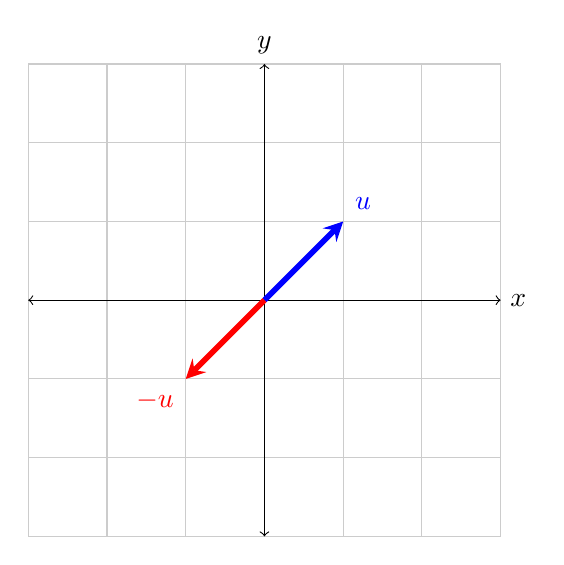
\begin{tikzpicture}
	\draw[thin,gray!40] (-3,-3) grid (3,3);
	\draw[<->] (-3,0)--(3,0) node[right]{$x$};
	\draw[<->] (0,-3)--(0,3) node[above]{$y$};
	\draw[line width=2pt,blue,-stealth](0,0)--(1,1) node[anchor=south west]{$\boldsymbol{u}$};
	\draw[line width=2pt,red,-stealth](0,0)--(-1,-1) node[anchor=north east]{$\boldsymbol{-u}$};
\end{tikzpicture}